--- |-
  \documentclass[sigconf]{acmart}
  \usepackage{graphicx}
\usepackage{hyperref}
\usepackage{todonotes}

\usepackage{endfloat}
\renewcommand{\efloatseparator}{\mbox{}} % no new page between figures

\usepackage{booktabs} % For formal tables

\settopmatter{printacmref=false} % Removes citation information below abstract
\renewcommand\footnotetextcopyrightpermission[1]{} % removes footnote with conference information in first column
\pagestyle{plain} % removes running headers

\newcommand{\TODO}[1]{\todo[inline]{#1}} \usepackage{endfloat} \renewcommand{\efloatseparator}{\mbox{}}
  \begin{document} \title{Big Data Analytics in Monitoring  Outdoor Air Quality}
  
  \author{Janaki Mudvari Khatiwada}
  \affiliation{% \institution{Indiana University, Bloomington} \streetaddress{P.O. Box 1212} \city{Bloomington} \state{Indiana} \postcode{43017-6221} } \email{jmudvari@iu.edu}
  
  
  
  
  \begin{abstract} Outdoor air pollution is one of the risk factors of public health. Air pollution adds burden to public health. Both developing and developed world use new technology and expertise to monitor outdoor air quality. United States Environmental Protection Agency (USEPA) collects outdoor air quality data from state, local and tribal agencies through outdoor air quality monitors across the country. The data get collected into the Air Quality System (AQS) database. This data can be used for variety of purposes such as education, research and regulatory. Data from this datamart is available for different timeseries like hourly, daily, weekly, monthly and yearly. It gives us a real picture of outdoor air quality and measurements of pollutants present in the air in a particular time period. The data can be used for comparing air quality among different regions, raise awareness to general public so that they can play a role in reducing household air pollutants, to see the trend of air pollutants at different time periods in a day or a season  and can also be combined with emissions data for comparative study. Data analysis of pollutants help identify pollution hot spots. Since air quality is vital for public health and environmental health, air quality monitoring possesses great significance from public health perspective. It is worth looking at recent average or maximum level of air quality index value for the pollutants described as criteria pollutants as described by World Health Organizations.
  
  \end{abstract}
  \keywords{i523, hid330, Outdoor Air Quality, Big Data, Particulate Matter }
  
  \maketitle
  
  
  \section{Introduction} Outdoor air is a valuable natural resource that is vital to the health and existence of human beings and other forms of life. The outdoor air not only has clean air but has presence of various pollutants. Several health research have revealed that air pollutants are contributing factors for lung cancer, cardiovascular disease, acute and chronic respiratory conditions. World Health Organization (WHO) in 2013 has assessed that air pollution is carcinogenic to humans \cite{www-who}. ``In 2012 WHO estimated that 72 percent of outdoor air pollution-related premature deaths were due to ischaemic heart disease and strokes'' \cite{www-who}. Being aware of this fact, governments along with the scientists and the environmentalists help make policies to combat air pollution. Each country has set their own standards for outdoor air quality to protect their citizen's health. Every nation's standards depend upon their economic, cultural, social and political needs. The United States enacted its Clean Air Act in 1970 and was amended in 1990 as a way to set stage for combating air pollution challenges \cite{epa-gov}. Since then, the country has made a lot of progress in improving air quality while sustaining a constant economic growth. Today, United States, European nations, India, China and other developing countries monitor outdoor air quality and use the collected data for identifying the particles present in the air, their contribution to various health problems, their sources, health research and also to find out the solutions to minimize their production level.
  Thousands of air quality monitors are placed  across the united States including US Virgin Islands and Puerto Rico live stream outdoor air quality data to a national air database system called Air Quality System (AQS). As a result big outdoor air data is generated constantly everyday. Air Quality System database is a national database where state, local and tribal agencies submit all of the data collected from thousands of air quality monitors across the United States. Besides air data, AQS database system has weather and emissions data. Emissions data provides data from vehicular, industrial and powerplants emissions records. Weather plays an important role in the quality of outdoor air. For example, high wind may disperse concentration of chemical particles. AQS database also called AQS Data Mart, has summary of yearly air quality data since the year of 1957. These data give an understanding of outdoor air quality and different particles present in the air and their sources. Source of air particles can be natural or human generated. Pollen, smoke from wildfires, mold, dust are some of the natural air pollutants. Similarly, emissions from power--plants, industries and vehicles, different substances and solutions that human have generated for various purpose are human generated air pollutants.
  To set standard for air quality, Air Quality Guidelines was published by WHO in 1987 and have been revised in 1997 \cite{who-health-topics}. WHO guidelines set an international standard for air quality based on which countries around the world set their own standards to achieve the goal set by WHO. Nitrous Oxide (NO2), Sulphur dioxide (SO2), Carbon Monoxide (CO), ground level Ozone, Particulate Matter (PM) among others, are some of the common hazardous air pollutants. Based on the value of Air Quality Index (AQI), USEPA has classified Outdoor air quality as 'Good', 'Moderate', 'Unhealthy for sensitive Groups', 'Unhealthy', 'Very Unhealthy' and 'Hazardous' \cite{airnow-gov}. The AQI value range from 0 to 500. The agency has assigned colors ('Green', 'Yellow', 'Orange', 'Red', 'Purple' and 'Maroon' respectively) to each of the air quality categories \cite{airnow-gov}. It is shown in figure \ref{AQI}.
  \section{Big Data and Outdoor Air Quality} In US there are about 4,000 outdoor air quality monitors operated by state environmental agencies \cite{outdoor-air}. They constantly collect air data on harmful suspended particles present in the air and send them to a national database center which is AQS database. EPA has air quality database from last 27 years from around the states \cite{googlecloud}. The data contains valuable information about the concentrations of different air pollutants in different time series; hourly, daily, weekly and yearly. Besides air quality data, AQS database also contains emissions data and weather data which are vital to the outdoor air air quality. Emissions data is basically data from vehicular and industrial emissions. They help to  understand the source of different air pollutants and their role in air quality as well as they can be used for furthering research in limiting their emissions. Yearly summary data of AQS Data Mart can also be used to see the progress made in reducing harmful air pollutants over the years. For example, NPA reported that emission of SO2 has reduced by 73 percent from 1990 to 2011 which is resulted primarily from electric utilities. Study of Emissions and air quality data gives an insight into the source of air pollutants and scientists can use these data to build a better industrial and vehicular models that reduces the emissions of pollutants. Similarly policy makers set vehicle emissions standards and industrial waste management.
  India and China, two bigger economies in the world are battling worst air pollution. In recent years IBM is doing collaborative work with local authorities to combat air pollution in cities like Delhi, Beijing and Johannesburg by providing its data analysis platform called `Green Horizons' \cite{www-huffingtonpost-com}. The platform uses machine learning tools to analyze past weather forecasts data along with near real time data from optical sensors, air quality monitors and satellites to understand past forecasting models and build a better prediction models for future forecasts \cite{www-huffingtonpost-com}. This prediction model helped Beijing enforce air quality control measures on traffic, construction and industry.
  Weather directly affects outdoor air quality. For example in a windy day PMs can easily be spread in a neighboring regions and high temperatures increases ground level ozone \cite{www-huffingtonpost-com}. Similarly, another example of relationship between big data analysis and air pollution is use of Microsoft's tools in incorporating Beijing's outdoor air data collected from conventional monitors along with data from ``environmental monitoring stations, traffic systems, weather satellites, topographic maps, economic data, and even social media '' \cite{spectrum-ieee}.
  Furthermore, `OpenAQ' is another platform besides EPA--AQS repository, which holds and hourly updates near--live air quality data from around the world. It claims to have ``collected 133,494,377 air quality measurements from 8,054 locations in 62 countries. Data are aggregated from 98 government level and research-grade sources'' \cite{googlecloud}. The platform helps general public identify global hotspots for poor air quality and allow to have a look at the outdoor air quality where they live \cite{googlecloud}. There is another open forum site called `Air--Now International' where users from around the world can participate in sharing and information about air quality data. ``It is an international version of USEPA's air now system''\cite{air-quality}.
  
  \section{Air Pollutants} EPA has prioritized six major air pollutants that are commonly found all over the US. They pose significant threat to public health and environment.  They are called `Criteria Pollutants' and they are ground level ozone, fine particles or particulate matter (PM 2.5 and PM 10), nitrogen dioxide, sulphur dioxide, lead and carbon monoxide \cite{epa-gov}. WHO has set the guidelines for each of these pollutants as shown in figure\ref{WHOGuidelines}.
  \begin{figure}[htb] 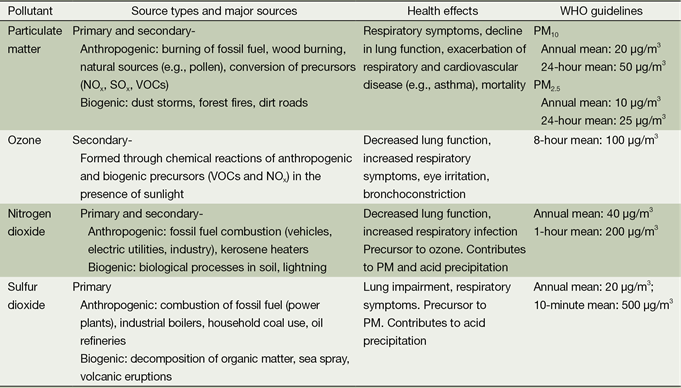
\includegraphics[width=1.0\columnwidth]{images/SourceandHealthEffects.png} \caption{WHO Guidelines Source And Health Effects \cite{guidelines}} \label{WHOGuidelines} \end{figure} PM 2.5 are particles less than or equal to 2.5 micrometers in diameter while PM 10 are particles less than or equal to 10 micrometers. ``Sulfate, nitrates, ammonia, sodium chloride, black carbon, mineral dust and water are the main components of PM '' \cite{www-who}. These components combine with each other to form variety of mixtures in the air and can easily enter our lungs. Longer exposure to these substances increases the risk of lung cancer and cardiovascular disease \cite{www-who}.
  Data on emissions from powerplants, industries and motor vehicles shows that emitted pollutants like various volatile substances and various forms of nitrogen oxides (NO2) are responsible in the formation of ground level ozone. Chemical reactions between these substances create ground level ozone directly in the air \cite{epa-gov}. Chest pain, coughing, throat irritation and inflammation are common problems caused by ozone air pollution. The main source of NO2 is emissions from heating, power generation and engines in vehicles and ships. SO2 is another air pollutant produced mainly from burning of fossil fuels. longer exposure to this pollutant causes inflammation of respiratory tract \cite{www-who}. The data on these pollutants have been regularly analyzed to see their trend. They have also been used in health research to have an understanding of their impact on people's health. Keeping track of problems and source of problems help us in keeping problem at check. Some air pollutants are characterized as hazardous or toxic air pollutants. Some of the examples include benzene, cadmium, mercury, lead and asbestos.
  \section{Health Hazards} Air pollutants, such as  hazardous air particles can easily reach our lungs when we breathe. The effect is itchy, irritated throat, nose and inflammation of respiratory tract. Pollutants such as PM 20 block our airtubes. These pollutants badly affects people with asthma and bronchitis. WHO had estimated that in 2012, 3 million premature deaths worldwide due to outdoor air pollution, particularly due to exposure to particulate matter of 10 microns or less \cite{www-who}. And in 2014 WHO has reported 7 million premature deaths worldwide \cite{www-who}. Other pollutants such as lead, pesticides, arsenic also called as toxic pollutants are carcinogenic hence are responsible for lung cancer which is one of premature deaths. Carbon monoxide a very common air pollutant generated by combustion has been called a silent killer. Its health effects include nausea, vomiting and reduced neuro and cardiovascular behavior as it blocks oxygen transfer inside the body.
  
  \section{Air Quality Index} AQI is the index, for five major air pollutants discussed above, calculated by EPA. Generally AQI 100 is the acceptable index set by EPA to protect public's health and it ranges from 0 to 500 \cite{airnow-gov}. The higher the value of AQI, greater is the pollution level and greater is the health risk. Based on hourly data collection from air quality monitors, stakeholders can constantly monitor AQI value in their cities or respective location. So weather channels in different media outlets such as local radio, television stations and newspapers also report about AQI index in order to inform general public about air quality in their area. Figure \ref{AQI} shows the AQI classification for each pollutant as recommended by WHO and implemented by U. S. EPA.
  \begin{figure}[htb] 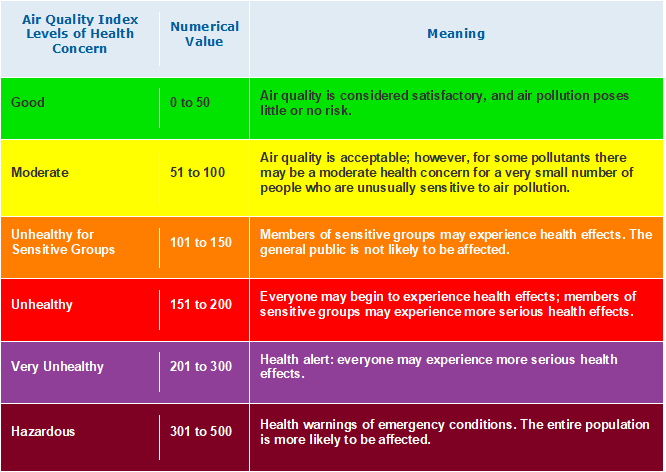
\includegraphics[width=1.0\columnwidth]{images/AQiclassification.png} \caption{Air Quality Index \cite{airnow-gov}} \label{AQI} \end{figure}
  \section{Outdoor Air Quality Monitoring Stations} Outdoor(Ambient) air quality monitors are specified based on the significance of monitoring a particular pollutant \cite{air-quality}. The purpose might be to protect public health or environment in a densely populated areas. They might be stationed nearby, schools, hospitals, parks and recreational areas. While they are operated by several different agencies they are regulated by U. S. EPA. According to EPA these stations should meet all the requirements for designs and operations as regulated by EPA themselves. These stations not only provide data on air quality they help in evaluating the effectiveness of programs and policies on emissions control.
  
  \section{WHO Guidelines and Clean Air Act} WHO guidelines for air quality is applied worldwide. This guidelines was revised in 2005 \cite{www-who}. The guidelines set standards for different air pollutants. According to the guidelines which is based on scientific evidence WHO has set standards for Ozone (o3), SO2, NO2 and PM. WHO guidelines try to limit the lowest possible values for these pollutants. For example WHO limit values for PM 2.5 is 10 micrograms per cubic meter is annual mean and 25 micrograms per cubic meter is 24-hour mean and limit value for PM10 is 20 μg/m3 annual mean and 50 μg/m3 24-hour mean \cite{www-who} \ref{WHOGuidelines}. ``The 2005 WHO Air quality guidelines'' offer global guidance on thresholds and limits for key air pollutants that pose health risks. The Guidelines indicate that by reducing particulate matter (PM10) pollution from 70 to 20 micrograms per cubic metre, we can cut air pollution-related deaths by around 15 percent \cite{www-who}.
  United States' Clean Air Act (CAA), first enacted in 1970 and with major revisions in 1990, is a federal law which is defined as ``The Act that regulates air emissions from area, stationary, and mobile sources'' \cite{epa-gov}. CAA  . EPA is the administrator of CAA \cite{wikipedia-org}. As required by law, EPA regulates emissions standards for vehicles, industries, aircrafts and powerplants among others in order to protect environment and public health. Today, with the availability of new technology and analytical tools air quality data from the monitors across the regions can be accessed in an instant and can be analyzed for daily reporting. Based on daily AQI value, respective authorities can take appropriate actions to save outdoor air quality in areas where pollution level is insignificant and to identify measures to be taken in areas where qir quality is poor.
  \section{Methods} \subsection{Air Quality Dataset} Outdoor air quality data sets are available in the USEPA.gov website called 'Air Data'. The data on 'Air Data website comes from AQS database where outdoor air data generated from thousands of air quality monitors from all over the country is collected. As mentioned, all states, local and private monitoring agencies send outdoor pollutants concentrations measurement data to the AQS database \cite{epa-gov}. Besides, Air Data there are other sources of data as well, they are briefly discussed below; 'Air Now' which has air quality forecasts and real--time data in visual format. \begin{itemize} \item `AirCompare' that has data about Counties' AQI summaries. \item `AirTrends' data is about trends of air quality and emissions. \item `Air Emissions Sources' has emissions data with national, state and county--level  summaries for criteria pollutant emissions. \item `Remote Sensing Information Gateway (RSIG)' that has air quality monitoring, monitoring and satellite data. \end{itemize}
  Air Data datasets  have raw dataset,  AQI summary datasets. Summary reports consists of AQI report which displays a yearly summary of AQI values in a countty or city or Core Based Statistical Area (CBSA). The AQI values are summarized by maximum percentile and median and count of days in each AQI category andteh count of days when AQI could be attributed to each criteria pollutant \cite{epa-gov}.
  `` Quality Statistics Report has yearly summaries of air pollution values for a city or county. It shows the maximum values reported during the year by all monitors in CBSA or county'' \cite{epa-gov}.
  Monitor Values Report that has yearly summary of the measurements at individual monitors and has descriptive information about the site \cite{epa-gov}.
  Monitor Values Report-Hazardous Air Pollutants that shows HAPs summary data for individual monitoring sites \cite{epa-gov}.
  Air Quality Index Daily Values Report that has information about AQi values for specified year and location \cite{epa-gov}.
  The data set that is being used for this paper is ``Daily AQI By CBSA 2016'', from EPA's air data website. Air data has different categories of outdoor air quality data. There are datasets with hourly as well as monthly datasets broken down by single criteria pollutant or 'Hazardous Air Pollutants' (HAPs). There are county level pollutants concentration measurements data sets or datasets by monitors and stations and datasets for grouped by ``Core Based Statistical Area'' (CBSA).
  CBSA is designed by Office of Management (OMB) as a geographical area that consists of one or more than one counties and similar surroundings that are associated with at least one core urbanized area of at least 10,000 population plus adjacent counties which are associated with each other in terms or social, economic and daily commutes \cite{www-census-gov}. CBSA collectively refers to Metropolitan and Micropolitan statistical areas. ``OMB defined Metropolitan and Micropolitan statistical areas in 2003 based on application of the 2000 standards with Census 2000 data. It became effective in 2003'' \cite{www-census-gov}. There are 922 CBSAs in total \cite{www-census-gov}. Metropolitan statistical areas are urbanized areas with population of 50,000 and its adjacent areas  while Micropolitan statistical areas are areas with population of at least 10000 or less than 50,000 \cite{www-census-gov}.
  CBSA AQI datasets fits the scenario for monitoring outdoor air quality. Because the designed statistical areas are significantly populated along with higher concentrations of motor vehicles running, higher number of day to day activities, less natural habitats or and most of the areas are within industrial areas and powerplant generators. Also, t First look at the dataset give a general information about AQI value of each 'Criteria Pollutant' for a day in a year of each monitoring stations in CBSAs.
  \subsection{Data Extraction and Data Cleaning} The comma separated dataset ``daily aqi by cbsa 2016'' was downloaded from data source ``https://aqs.epa.gov/aqsweb/airdata''. The dataset shows AQI value of each ``criteria pollutants'' for each CBSA recorded per day per station for the year 2016. Criteria pollutants recorded in the dataset are, PM2.5, PM10, Ozone, SO2, NO2 and CO. It also has a column for number of stations for each DBSA and location of the monitoring stations per CBSA.
  Criteria pollutants recorded in the dataset varies within each CBSAs depending on their significance in the region or monitoring stations. Similarly, Record date per station per CBSAs is not continuous, there are records for date january 1 2016 and the next date is January 3 or 6 and so on. This random pattern is seen in the whole data set. Also, number of monitoring stations varies per CBSAs.
  Using jupyter notebook with python2.7 as the interpreter, the dataset is cleaned and converted  into pandas dataframe for analysis and manipulation. Jupyter Notebook is an open source web application which is powerful in data cleaning, manipulation, data analysis and visualizations. The notebook is not sufficient in itself for a variety of data manipilations, it need to have all sorts of python packages as per requirement of data analysis. Matplotlib, pandas, numpy and pandas datetime are the packages used for air quality data analysis.
  
  \section{Analysis} The requirements for the analysis are python's jupyter notebook and the packages pandas, matplotlib and numpy. Using the pandas dataframe, average AQI value is calculated for each `Defining Parameter' grouped by CBSA.  Since AQI value determines the level of risk factor as shown in figure \ref{AQI}, it is worth calculating the mean of that value which helps in determining which CBSA is affected by which `defining Parameter'. It also helps identify the source of that defining particle so that responsible stakeholders can take required actions to solve the problem. The purpose of using the data set is to find out level of AQI per CBSA  for the year 2016. The reason of using 2016 data set is it the most recent complete set of data for a year. While 2017 data set would have been the most recent look at AQI level in the United States but as of this analysis the 2017 data set contains air quality data until the month of May 2017. This data set wold be completed as a full years data only in the upcoming spring \cite{outdoor-air}.
  Simple statistical measures such as mean, maximum, count and minimum value for any variable provides some insight into a general knowledge about the variable.
  
  
  
  
  
  
  
  
  
  
  \section{Conclusion} There is tremendous application prospects of using MQTT protocol in big data and edge computing. Edge computing, being a new  development in data analytics,
  
  \begin{acks}
  The author would like to thank Dr. Gregor von Laszewski for his support and suggestions to write this paper.
  \end{acks}
  \bibliographystyle{ACM-Reference-Format} \bibliography{report}
  
  
  \end{document}
